% Change to use the correct class file for your paper.
\documentclass[10pt]{report}
%\nocopyrightspacetrue

%\pagenumbering{arabic}

\usepackage{amsfonts}
\usepackage{array}
\usepackage{booktabs}
\usepackage{color}
\usepackage{colortbl}
\usepackage{endnotes}
%\usepackage[cm]{fullpage}
\usepackage[margin=0.5in]{geometry}
\usepackage{graphicx}    % For importing graphics
\usepackage[draft]{hyperref}    % Creates hyperlinks from ref/cite
%\usepackage{hyperref}    % Creates hyperlinks from ref/cite
\usepackage{multirow}
\hypersetup{pdfstartview=FitH}
%\usepackage{subfig}
\usepackage{subfigure}
\usepackage{tabularx}
\usepackage{url}         %
\usepackage{xspace}
%\usepackage[bf,skip=5pt]{caption}
\usepackage[skip=5pt]{caption}
\usepackage{comment}
\usepackage{amssymb}
\usepackage{amsmath}
\usepackage{amsfonts}
\usepackage{wrapfig}
\usepackage{listings}

%\usepackage{xcolor}
\usepackage{colortbl}
\usepackage{threeparttable}
\usepackage{soul}
\usepackage{enumitem}

\DeclareCaptionType{copyrightbox}

\newlength\SUBSIZE

\renewcommand{\arraystretch}{1.2} % Space out rows in tables

\newcommand{\projname}{Super Super Sweet (S$^3$) Project Name\xspace}
\newcommand{\ra}{$\rightarrow$\xspace}

\setlength\paperheight {11in}
\setlength\paperwidth {8.5in}

% Set the graphics path
\graphicspath{{../figs/}{../images/build/}}
%\DeclareGraphicsExtensions{.pdf,.png,.jpg}


% No space between bibliography items:
\let\oldthebibliography=\thebibliography
  \let\endoldthebibliography=\endthebibliography
  \renewenvironment{thebibliography}[1]{%
    \begin{oldthebibliography}{#1}%
      \setlength{\parskip}{0ex}%
      \setlength{\itemsep}{0ex}%
  }%
  {%
    \end{oldthebibliography}%
  }
\setlength{\parindent}{5mm}

\newcommand{\sdr}{$\mu$SDR\xspace}
\newcommand{\superscript}[1]{\ensuremath{^{\textrm{#1}}}}
\newcommand{\subscript}[1]{\ensuremath{_{\textrm{#1}}}}
\newcommand{\realtilde}{\raise.17ex\hbox{$\scriptstyle\sim$}}

\begin{document}

%\CopyrightYear{}
%\crdata{}
\clubpenalty=10000
\widowpenalty = 10000

\title{\sdr User's Manual\\ Version 0.1}
\author{Ye-sheng Kuo}
\date{Sep 2012}
\maketitle
\tableofcontents
\chapter{Overview}
\sdr is a software-defined radio based on Microsemi's SmartFusion. Unlike common FPGAs, the SmartFusion
is a device which incorporates a hard core ARM Cortex M3 and a flash-based FPGA. Flash-based FPGA
technology offers low static power, no reconfiguration in boot stage and memory retention when in
power down mode. These benefits make it a better candidate for low-power wireless research. We present
the \sdr, a true battery-powered SDR platform which is suitable for portable and deployable hand held
device research.
\section{Features}
\begin{enumerate}
	\item 2.4 - 2.5~GHz ISM band
	\item Dual channel 80~MS/s, 8-bits ADC
	\item Dual channel 40~MS/s, 8-bits DAC
	\item 16~MB External PSRAM
	\item 8~MB External Flash
	\item $\pm$3~ppm TXCO
	\item Ethernet, USB interfaces
	\item 24 User defined IO, 8 LEDs and 4 switches
	\item Battery-powered
\end{enumerate}

\begin{figure}[h]
\centering
	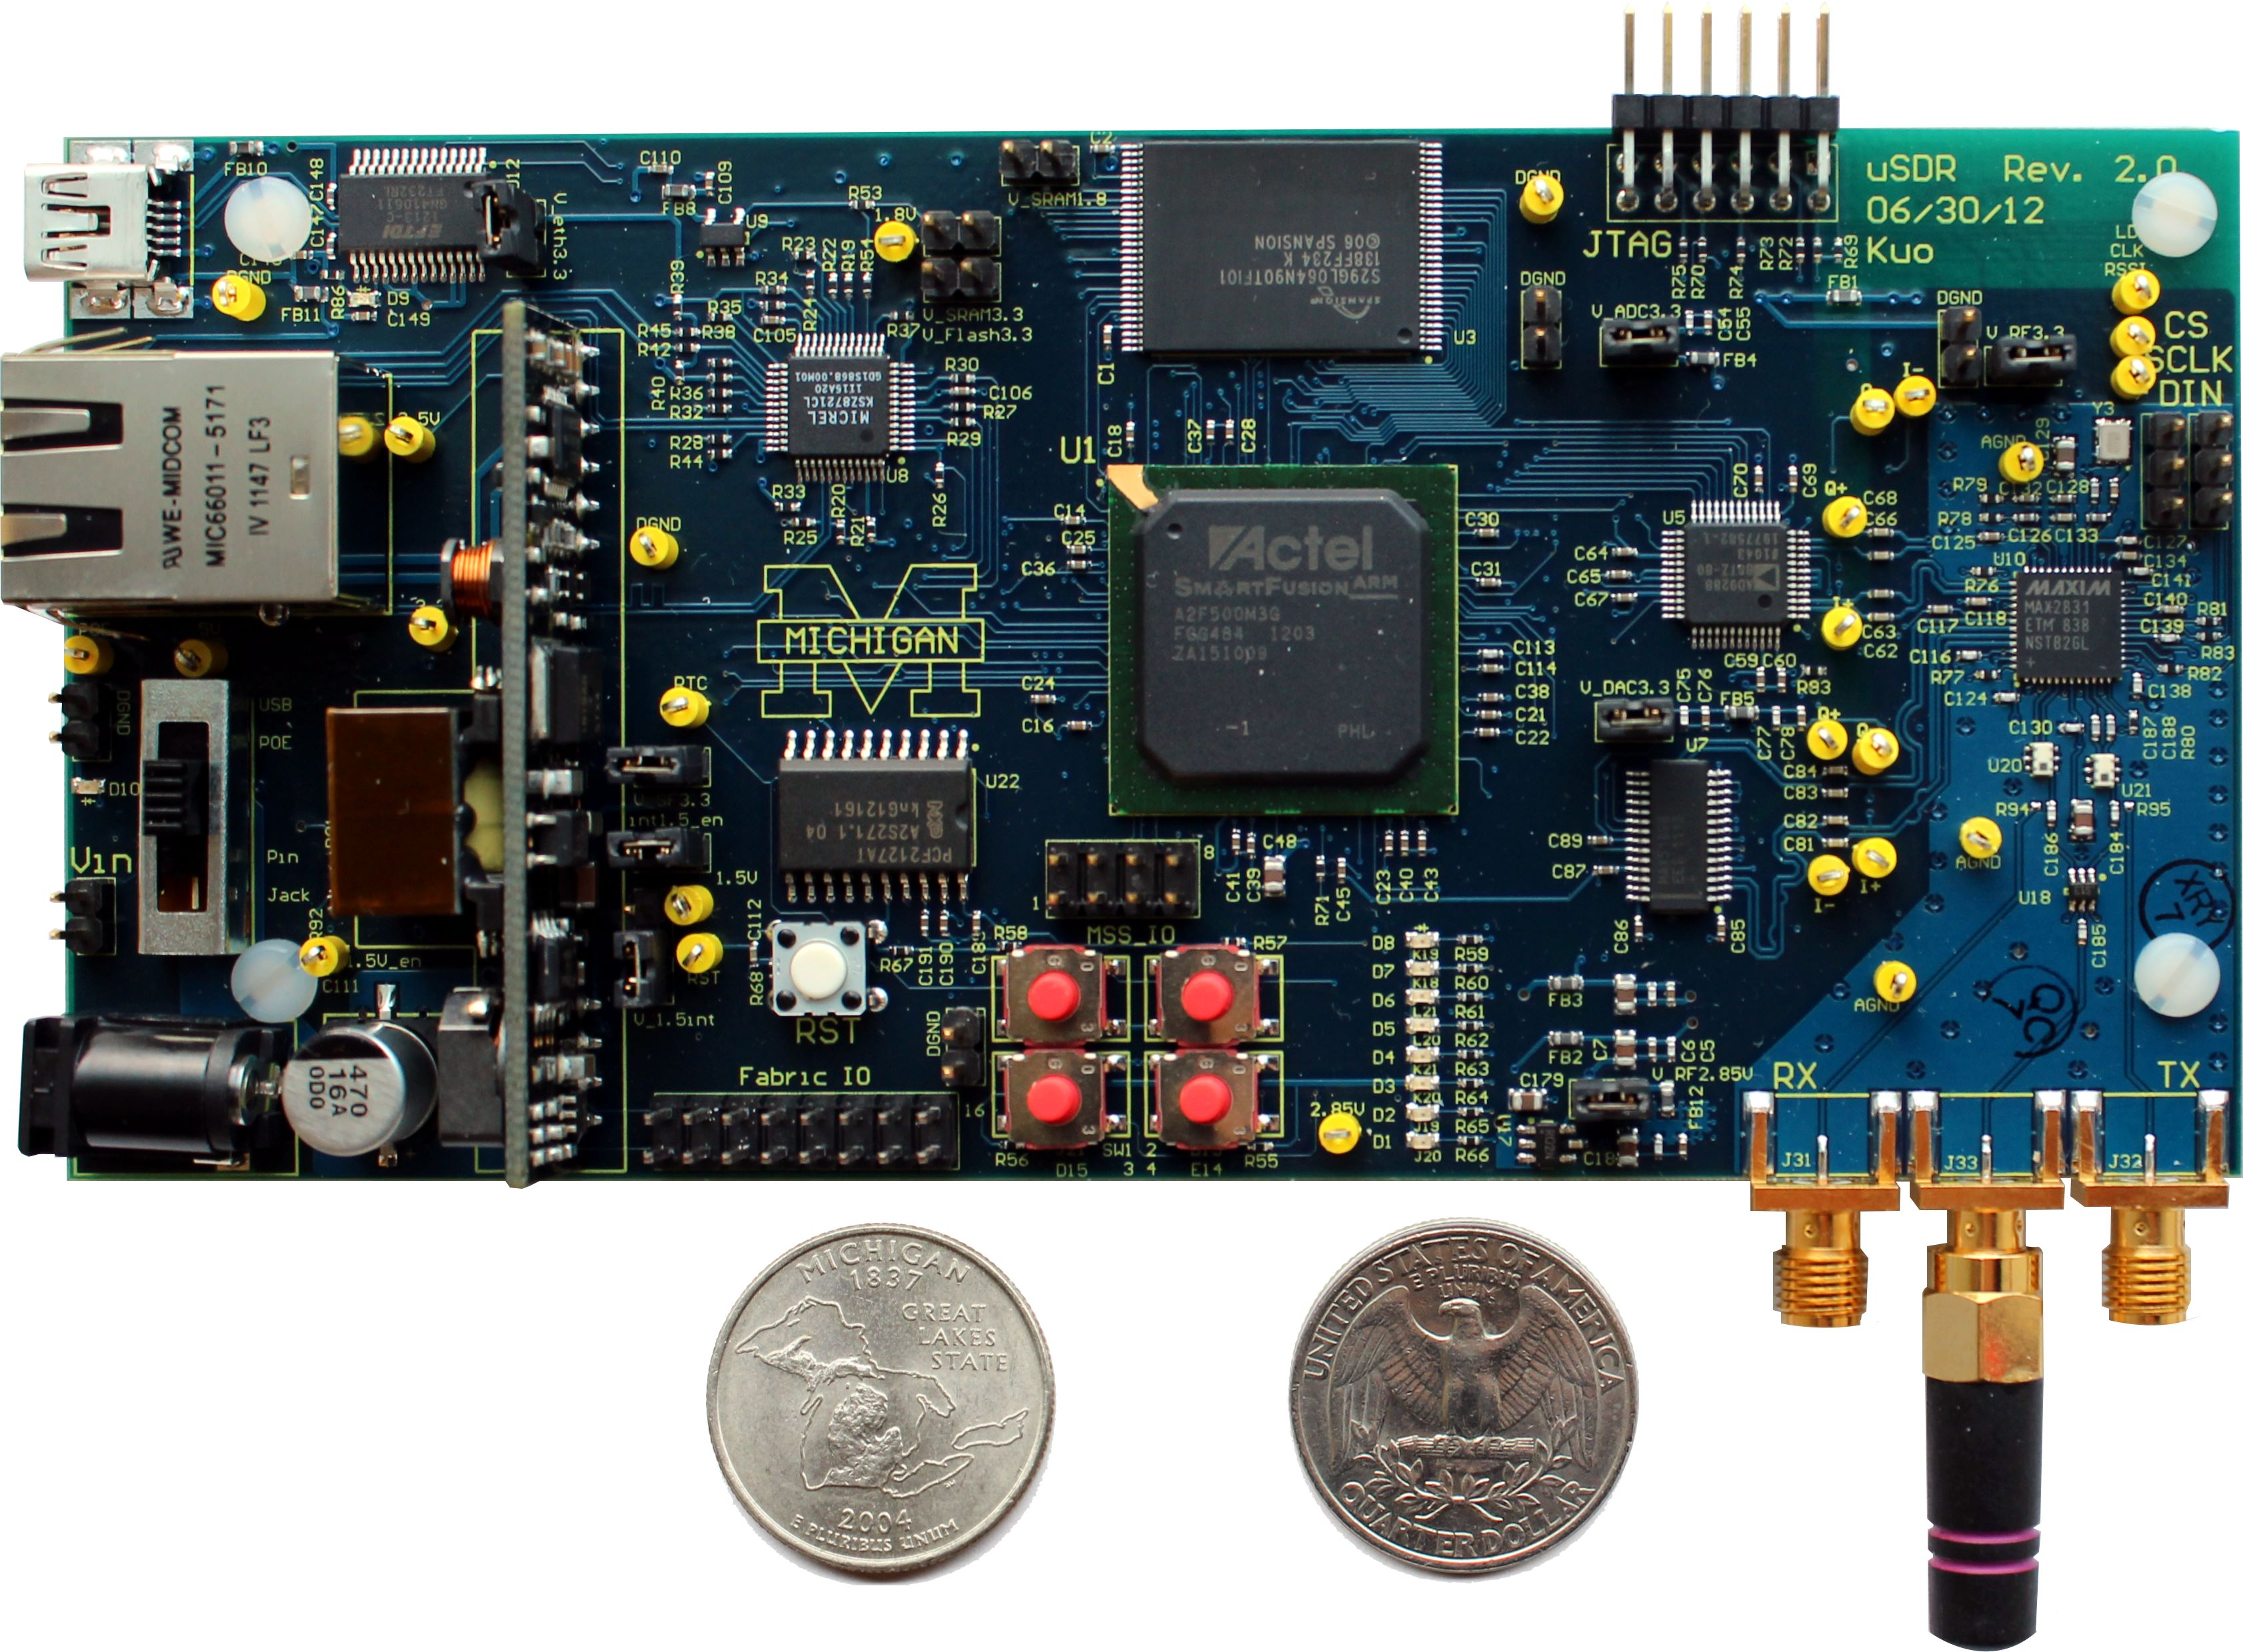
\includegraphics[width=0.6\columnwidth]{sdrv2_scale}
\end{figure}

\chapter{Hardware}

\hl{NOTE: needs a top level diagram. That would make the connections a lot easier to follow.}

\hl{IDEA: combine all of the IO connection tables into one super table so all wiring is in one spot.}

The major components of \sdr are the following:
\begin{description}
	\item[Microsemi Smartfusion] \hfill \\
	The procssing core of \sdr. It incorporates an
	analog computing engine, a flash-based FPGA and a hardcore ARM Cortex-M3.
	\item[MAXIM MAX2831] \hfill \\
	The MAXIM 2831 is a 2.4~GHz ISM band RF frontend. This
	chip integrates common RF blocks (power amplifier, filters, voltage
	control oscillator, etc.) into a single chip.
	\item[Analog Device AD9288] \hfill \\
	8-bits Dual channel high speed ADC. Three variants
	are available. The one which is currently employed on \sdr is 80~MSP/s.
	\item[MAXIM MAX5189] \hfill \\
	8-bits Dual channel 40~MHz DAC. Both channels share
	the same input but latching the data using different edges of clock input.
	\item[Micrel KS8721CL] \hfill \\
	100Base-TX Physical Layer Transceiver providing RMII interfaces to MACs
	and switches.
	\item[FTDI FT232R] \hfill \\
	USB to UART interface. It connects to the UART0 of SmartFusion device.
	\item[External Mem] \hfill \\
	\sdr has 2 external memories which are 16~MB PSRAM and 8~MB flash installed.

\end{description}

\section{Power}
\subsection{Power Rails}
\sdr uses many different power rails for many purposes. Every power rail is produced by an
LDO (Low Drop-Out regulator).
\begin{enumerate}
	\item 3.3~V, the major power supply for {\bf Smartfusion, ADC, DAC, RF, Ethernet,
	USB, RTC, PSRAM, and FLASH}
	\item 2.85~V, {\bf RF} only.
	\item 1.8~V, {\bf PSRAM} only.
	\item 1.5~V, {\bf Smartfusion(Core)} only.
\end{enumerate}

\subsection{Power Source}
\sdr can be powered by USB, PoE, exposed headers or power jack. A 4-way switch is used to select
the input power source.

\subsection{1.5V on-chip regulator}
The SmartFusion integrates a 1.5~V on-chip regulator. This regulator could be turned on
by triggering a specific IO or software interrupt. Similarly, this regulator could
be turned off by setting a specific register.

Jumper P15 (``int1.5\_en'') must be jumpered in order to enable the on-chip 1.5~V regulator. Jumper P16 (``V\_1.5int'')
is the 1.5~V power selector. Jumpering the upper 2 pins powers the \sdr using the external
regulator. In contrast, jumpering the bottom 2 pins causes \sdr to use the on-chip 1.5~V regulator.

\subsection{Enabling/Disabling Power}
\sdr offers many jumpers to separate the power domain across subsystems. User can
manually disconnect the power supplies by removing the jumpers. These jumpers also provide
convenient locations to measure the current
through a specific chip.

Note: 1.5~V and 3.3~V on SmartFusion and Ethernet are required
for the \sdr to operate properly.

\hl{NOTE: this needs to be further explained with a table of what jumpers power what.}

\section{RF Frontend}
The MAX2831 provides a 3-wire SPI interface as well as a 7-bit wide gain control bus.
Every register can be written through the SPI interface, however, the SPI interface doesn't allow
for reading the current registers' value. TX baseband gain, RX baseband gain and
RX LNA gain can be controlled using these registers and 7-bit bus. Since the SPI interface clocks
a single bit at a time, it has longer latency when setting the gain control than the 7-bit bus.
Therefore, AGC benefits from the parallel bus.
In order to enable the parallel bus gain control, registers 8 D12 and 9 D10
must be asserted. In the receiving mode, bits B7 and B6 control the LNA gain setting and bits B5\~{}B1
control the baseband VGA gain.

Two additional control wires (RX\textbackslash{}TX, SHDN) control the modes. Available
modes are listed in Table~31 in datasheet~\cite{MAX2831}.

The analog RSSI signal is connected to a low-power serial ADC~\cite{ADC081S101} that operates up to 1~MSP/s.
The maximum output of serial ADC is 223 (3.3~V) instead of 255. Therefore, the step size
of serial ADC is {\bf 14.8~mV}.

The MAX2831 separates the TX/RX path. Since it cannot fully duplex communication, an
RF switch~\cite{AS213} is used to allow a single antenna. If desired, users can
use separate antennas by applying the three small changes listed below.

{\bf Instructions for Using Separate Antennas:}
\begin{enumerate}[noitemsep]
	\item Remove C184, C186.
	\item Short R94, R95.
	\item Install antennas on J31, J33.
\end{enumerate}

\subsection{Test Points}
Various test points are available on \sdr. Analog signals include TX/RX I/Q channels, LD, CLK and RSSI.
P12, P13 (on the edge of \sdr) provide digital test points for SPI interface of MAX2831 and
ADC081S101.

\hl{NOTE: need a better table for this. It's not clear which pins exactly
correspond to which SPI signals.}

\subsection{IO connection}
MAX2831 interface
\begin{table}[h]
\centering
\begin{tabular}{|l|c|c|}
	\hline
	{\bf Name} & {\bf Physical Connection} & {\bf Direction}\\ \hline
	RX\textbackslash{}TX 	& L18 & Out\\ \hline
	SHDN 	& M18 & Out\\ \hline\hline
	\={CS}	& H20 & Out\\ \hline
	DATA	& J22 & In\\ \hline
	CLK		& L22 & Out\\ \hline\hline
	B1 (VGA, LSB) 	& D7 & Out\\ \hline
	B2 (VGA)		& E8 & Out\\ \hline
	B3 (VGA)		& C4 & Out\\ \hline
	B4 (VGA)		& C5 & Out\\ \hline
	B5 (VGA, MSB)	& D8 & Out\\ \hline
	B6 (LNA, LSB)	& C7 & Out\\ \hline
	B7 (LNA, MSB)	& C8 & Out\\ \hline
\end{tabular}
\end{table}

RSSI Serial ADC (ADC081S101) interface (SPI)
\begin{table}[h]
\centering
\begin{tabular}{|l|c|c|}
	\hline
	{\bf Name} & {\bf Physical Connection} & {\bf Direction}\\ \hline
	\={CS}	& H17 & Out\\ \hline
	DATA	& H22 & In\\ \hline
	CLK		& H18 & Out\\ \hline
\end{tabular}
\end{table}

\clearpage
\section{ADC}
Channels A and B of the AD9288~\cite{AD9288} are connected to the In-phase and Quad-phase channels of the MAX2831, respectively.
The input common-mode voltage of the AD9288 is 0.3$*$VDD which is 0.99~V. However, the common-mode
voltage of the MAX2831 is not able to be tuned to 0.99~V. A voltage reference chip, the MAX6061~\cite{MAX6061},
and a voltage divider are used to alter the common-mode voltage.

The output of the AD9288 on \sdr is pre-configured to 2's complement output. Therefore,
D7\subscript{A, B} are sign bits for each channel. Deassert signal S1 to put the AD9288 into
standby mode. More detail can be found in Table~4 in datasheet~\cite{AD9288}.

\subsection{IO connection}
\begin{table}[h]
\centering
\begin{tabular}{|l|c|c|}
	\hline
	{\bf Name} & {\bf Physical Connection} & {\bf Direction}\\ \hline
	D0\subscript{A} (I, LSB) 	& C21 & In\\ \hline
	D1\subscript{A} 			& D21 & In\\ \hline
	D2\subscript{A}				& B20 & In\\ \hline
	D3\subscript{A}				& C19 & In\\ \hline
	D4\subscript{A}				& G19 & In\\ \hline
	D5\subscript{A}				& F19 & In\\ \hline
	D6\subscript{A}	(I, MSB)	& G21 & In\\ \hline
	D7\subscript{A} (I, Sign)	& G20 & In\\ \hline\hline
	D0\subscript{B} (Q, LSB) 	& K17 & In\\ \hline
	D1\subscript{B} 			& J17 & In\\ \hline
	D2\subscript{B}				& F21 & In\\ \hline
	D3\subscript{B}				& F20 & In\\ \hline
	D4\subscript{B}				& G18 & In\\ \hline
	D5\subscript{B}				& G17 & In\\ \hline
	D6\subscript{B}	(Q, MSB)	& E18 & In\\ \hline
	D7\subscript{B} (Q, Sign)	& F17 & In\\ \hline\hline
	CLK							& A17 & Out\\ \hline\hline
	S1							& D18 & Out\\ \hline
\end{tabular}
\end{table}

\clearpage
\section{DAC}
Similarly, the MAX6061 voltage reference chip is deployed on the transmission path to pull the
common-mode voltage. The MAX5189~\cite{MAX5189} uses both edges of the clock to update both
channel outputs. The maximum clock input frequency of the MAX5189 is 40~MHz. The combination
of DACEN and PD determines the operation mode, more detailed information can be found
in Table~1 of the datasheet~\cite{MAX5189}.

\subsection{IO connection}
\begin{table}[h]
\centering
\begin{tabular}{|l|c|c|}
	\hline
	{\bf Name} & {\bf Physical Connection} & {\bf Direction}\\ \hline
	D0 (LSB)	& E1  & Out\\ \hline
	D1			& F3  & Out\\ \hline
	D2			& G4  & Out\\ \hline
	D3			& H5  & Out\\ \hline
	D4			& H6  & Out\\ \hline
	D5			& J6  & Out\\ \hline
	D6			& B22 & Out\\ \hline
	D7 (MSB)	& C22 & Out\\ \hline\hline
	CLK			& A18 & Out\\ \hline\hline
	DACEN		& F1  & Out\\ \hline\hline
	PD			& G2  & Out\\ \hline
\end{tabular}
\end{table}

\section{User's IO}
\sdr has eight user-defined LEDs and four push-button switches. The LEDs and switches are {\bf active low}. The LEDs/switches
are connected to the Fabric, however, users can route the connection to the MSS IO. In addition, two IO
banks also available on \sdr. A 16-pin wide interface is connected to the Fabric, whereas an 8-pin
bus is connected to fixed\footnote{GPIOs on Fabric are able to route to MSS IO Pads, however,
GPIOs on MSS cannot be routed to Fabric.}
MSS GPIOs. Libero SoC must be configured to enable the MSS GPIO.

\subsection{IO connection}
\begin{table}[h]
\centering
\begin{tabular}{|l|c|c|}
	\hline
	{\bf Name} & {\bf Physical Connection} & {\bf Direction}\\ \hline
	LED0 & J20 & Out \\ \hline
	LED1 & J19 & Out \\ \hline
	LED2 & K20 & Out \\ \hline
	LED3 & K21 & Out \\ \hline
	LED4 & L20 & Out \\ \hline
	LED5 & L21 & Out \\ \hline
	LED6 & K18 & Out \\ \hline
	LED7 & K19 & Out \\ \hline\hline
	SW1  & J21 & In	 \\ \hline
	SW2  & B19 & In	 \\ \hline
	SW3  & D15 & In	 \\ \hline
	SW4  & E14 & In	 \\ \hline
\end{tabular}
\end{table}

\clearpage

\begin{table}[h]
\centering
\begin{tabular}{|l|c|c|}
	\hline
	{\bf Name} & {\bf Physical Connection} & {\bf Direction}\\ \hline
	Fabric IO\subscript{0}	& N6 & In/Out \\ \hline
	Fabric IO\subscript{1}	& M6 & In/Out \\ \hline
	Fabric IO\subscript{2}	& P1 & In/Out \\ \hline
	Fabric IO\subscript{3}	& P2 & In/Out \\ \hline
	Fabric IO\subscript{4}	& N3 & In/Out \\ \hline
	Fabric IO\subscript{5}	& N2 & In/Out \\ \hline
	Fabric IO\subscript{6}	& M2 & In/Out \\ \hline
	Fabric IO\subscript{7}	& M1 & In/Out \\ \hline
	Fabric IO\subscript{8}	& M4 & In/Out \\ \hline
	Fabric IO\subscript{9}	& L3 & In/Out \\ \hline
	Fabric IO\subscript{10}	& L2 & In/Out \\ \hline
	Fabric IO\subscript{11}	& L1 & In/Out \\ \hline
	Fabric IO\subscript{12}	& L5 & In/Out \\ \hline
	Fabric IO\subscript{13}	& K4 & In/Out \\ \hline
	Fabric IO\subscript{14}	& L6 & In/Out \\ \hline
	Fabric IO\subscript{15}	& K6 & In/Out \\ \hline\hline
	MSS IO\subscript{0}		& T3 & In/Out \\ \hline
	MSS IO\subscript{1}		& V3 & In/Out \\ \hline
	MSS IO\subscript{2}		& U3 & In/Out \\ \hline
	MSS IO\subscript{3}		& T4 & In/Out \\ \hline
	MSS IO\subscript{4}		& AA2& In/Out \\ \hline
	MSS IO\subscript{5}		& AB2& In/Out \\ \hline
	MSS IO\subscript{6}		& AB3& In/Out \\ \hline
	MSS IO\subscript{7}		& Y3 & In/Out \\ \hline
\end{tabular}
\end{table}

\section{TCXO}
The PCF2127A~\cite{PCF2127A} is a temperature-compensated low-frequency oscillator. It provides $\pm$3ppm stability
over a wide range of temperature and it replaces the 32.768~KHz crystal oscillator \hl{ replaces what crystal oscillator?}.
The configuration
interface is connected to the MSS SPI bus 1\footnote{It's a fixed connection and needs to be initiated in
Libero SoC MSS configuration tool.} and the interrupt is connected to a Fabric IO. A external coin-cell
battery provides an additional power source for the PCF2127A. \sdr automatically switches the power source if V\subscript{DD} is
less than a certain threshold. \hl{ Less than what threshold?}
\subsection{IO connection}
\begin{table}[h]
\centering
\begin{tabular}{|l|c|c|}
	\hline
	{\bf Name} & {\bf Physical Connection} & {\bf Direction}\\ \hline
	INT & B7 & In\\ \hline\hline
	D\subscript{IN} & T17 & Out\\ \hline
	D\subscript{OUT} & V19 & In\\ \hline
	CLK & AA22 & Out\\ \hline
	\={CS} & W21 & Out\\ \hline
\end{tabular}
\end{table}

\clearpage
\section{Ethernet}
\subsection{Power over Ethernet}
\sdr can be powered by Ethernet. The PoE module on the \sdr is the AG9205S~\cite{AG9200S} and it provides up to
13~W power output. The default power setting on \sdr is configured to 3.84~W, which is equivalent to 768~mA
maximum current. The setting can be changed by replacing the configuration
resistor R50. More power ratings are available in Table~2 in datasheet~\cite{AG9200S}.

\subsection{Disabling KSZ8721}
The Ethernet transceiver KSZ8721 on \sdr is enabled by default. The transceiver draws about 50~mA
when in an idle state. In low-power applications when the transceiver is not needed, it can be turned off\footnote{
The Ethernet subsystem cannot be disabled by removing the jumper P7 (``V\_eth3.3''). Doing this results in the SmartFusion working
improperly.} by patching the \sdr.

{\bf Instructions to Disable the KSZ8721 Ethernet Module:}
\begin{enumerate}[noitemsep]
	\item Remove R36.
	\item Put 10~K resistor on R33.
\end{enumerate}

\subsection{IO connection}
\begin{table}[h]
\centering
\begin{tabular}{|l|c|c|}
	\hline
	{\bf Name} & {\bf Physical Connection} & {\bf Direction}\\ \hline
	CLK (50~MHz) & E3 & In \\ \hline
\end{tabular}
\end{table}

%\section{USB}
%\section{External Memory}

\chapter{802.15.4 Application}

\section{Fabric Architecture}
802.15.4 application integrates the basic transceiver functionality into Fabric. 
User can initiate transmission or receiving by simply writing to specific registers.
Figure~\ref{fig:radio_state} is a simplified model of state machine. The details for each state
will be discussed in following.
\begin{figure}[t]
	\centering
	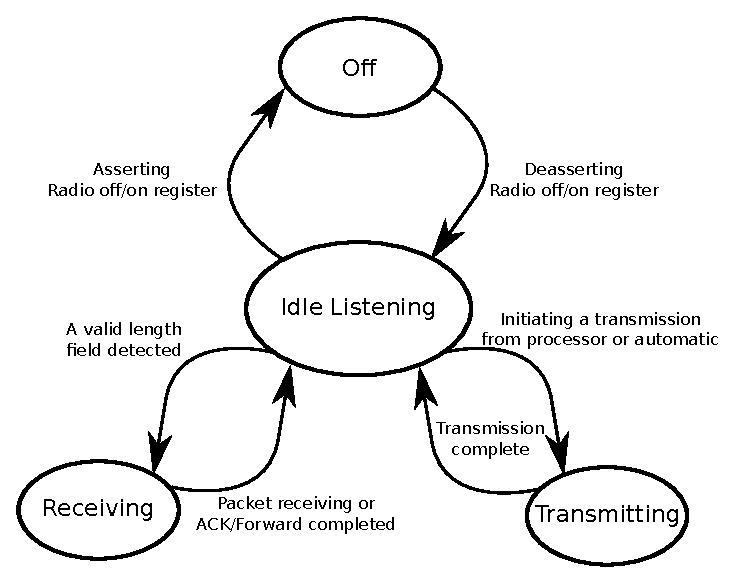
\includegraphics[width=0.6\columnwidth]{radio_state}
	\caption{Simplified radio state diagram}
	\label{fig:radio_state}
\end{figure}

\begin{figure}[h]
\centering
	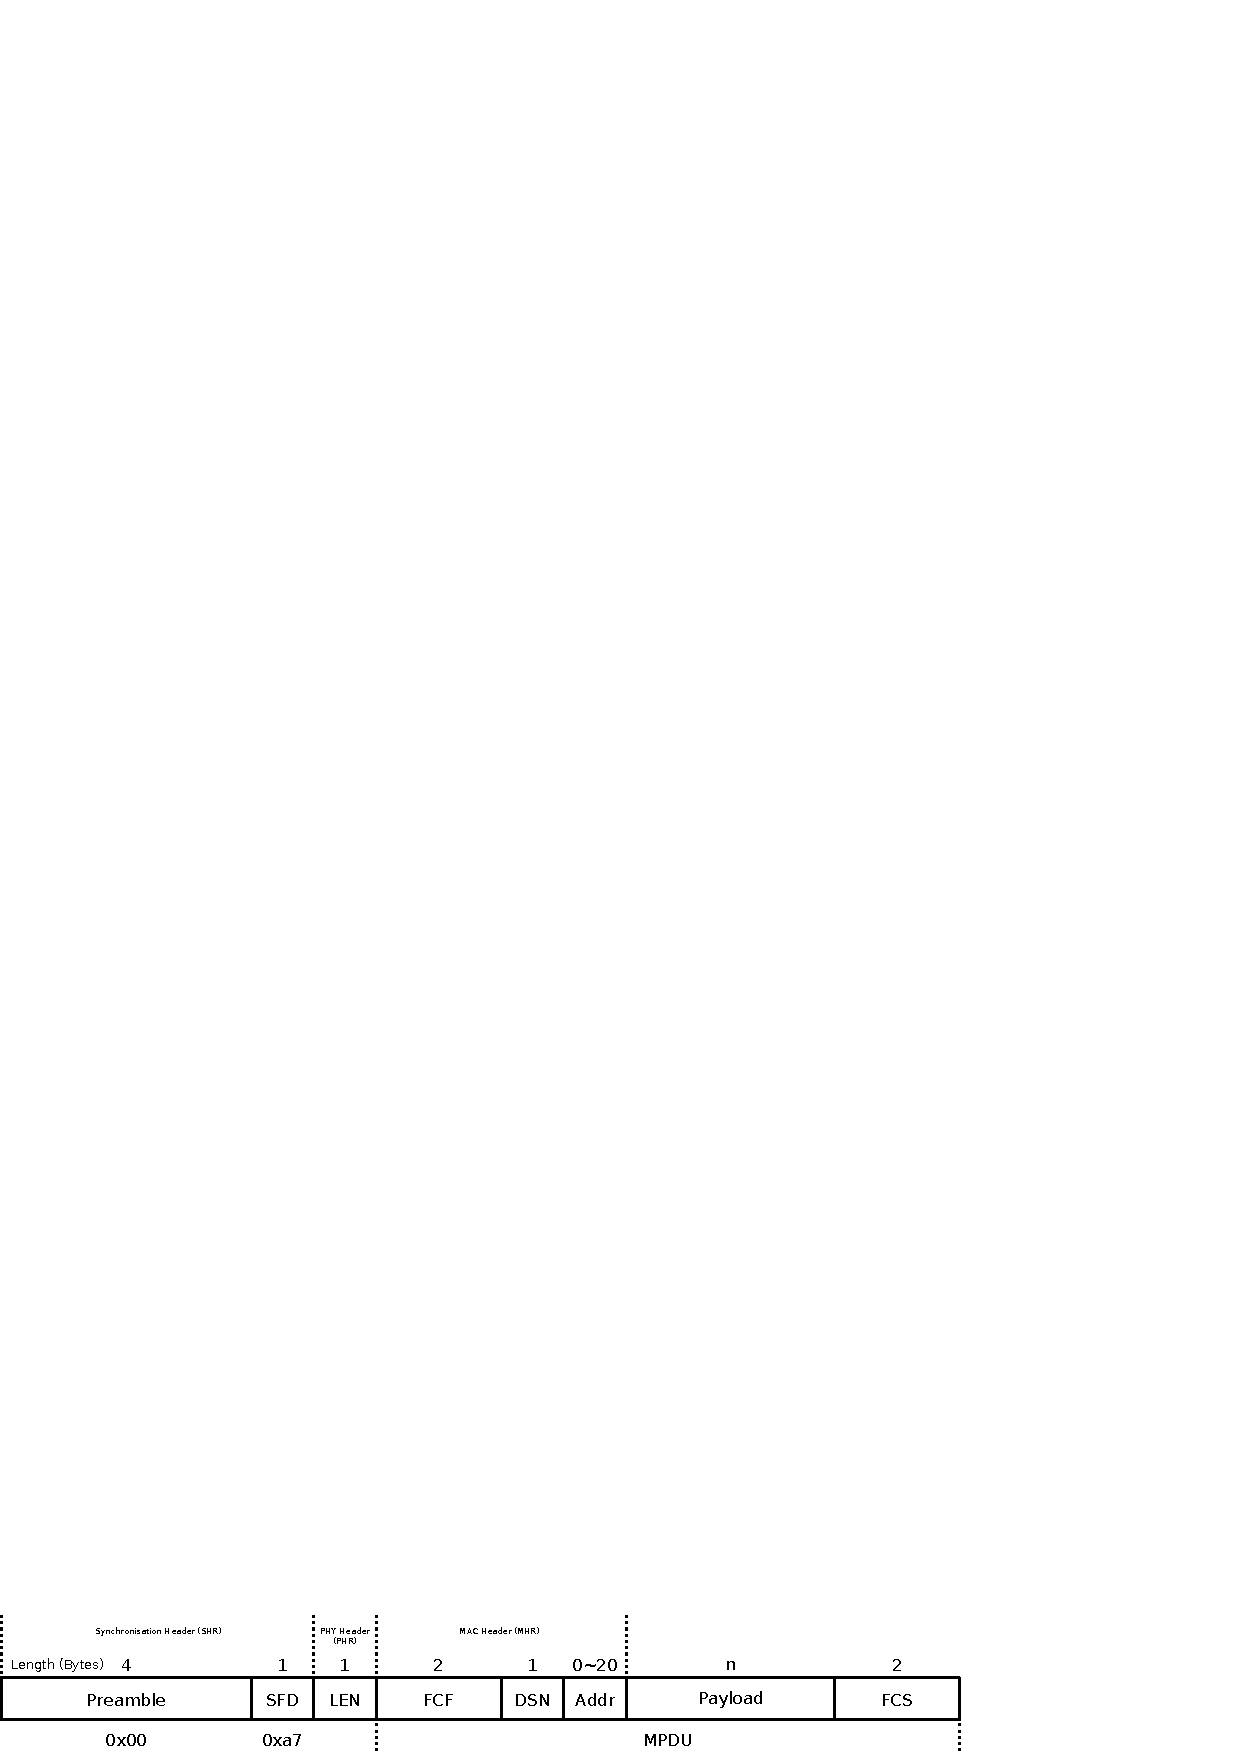
\includegraphics[width=0.9\columnwidth]{frame_format}
	\caption{Frame format of a 802.15.4 packet}
\end{figure}

\subsection{Radio states}
\subsubsection{Off Mode}
\hangindent=\parindent
\hangafter=0
Once the \sdr exits global system reset, radio starts with {\bf Off} state.
In this state, the radio peripherals (RF frontend, ADCs and DAC) are in the 
lowest power state to save energy. Radio exits this state if the following event
has been triggered.
\begin{description}
	\item[1. Deasserting Radio off/on register:] Radio exits {\bf Off} mode
	and a series of hardware initializations take place at this stage. Once the
	discrete chips are ready, the radio arrives {\bf Idle Listening} mode.
\end{description}

\subsubsection{Idle Listening Mode}
\hangindent=\parindent
\hangafter=0
In this mode, radio has RF frontend on in RX mode and ADCs actively running. Radio keeps
decoding wireless signal and trying to identify any incoming packet. In addition, radio
is ready to initiate a packet transmission in this state. Radio exits this state if the 
following event has been triggered.
\begin{description}
	\item[1. Asserting Radio off/on register] Radio turns-off all peripherals and 
	entering the {\bf Off} mode to save energy.
	\item[2. Incoming packet detected] Once a valid length field has been decoded, 
	radio enters {\bf Receiving} mode to ensure receiving a completed packet.
	\item[3. Initiating packet transmission] The start transmission command from processor
	or Fabric itself trigger the radio into {\bf Transmission} mode.
\end{description}

\subsubsection{Receiving Mode}
\hangindent=\parindent
\hangafter=0
Since the radio is not transmitting in this state, DAC has been turned-off to save energy.
In the mean time, RF frontend and ADCs actively running and receiver blocks decode
wireless data. Receiver performs a basic frame filtering and storing the incoming bytes
into fifos. Radio exits this state if the following event has been triggered.
\begin{description}
	\item[1. Receiving completed] A packet has been received completely and this packet
	doesn't request ACK nor Forward. Radio backs to {\bf Idle Listening}.
	\item[2. ACK/Foward completed] Radio backs to {\bf Idle Listening} if ACK/Forward\footnote{
	802.15.4 standard requires 192~$\mu$s between transmissions (ACK/Forward). The 
	timing requirement is taken care in hardware.}
	packet has been transmitted completed.
\end{description}

\subsubsection{Transmission Mode}
\hangindent=\parindent
\hangafter=0
In transmission mode, ADCs has been turned-off and the receiver is put into reset. Transmitter
starts reading the data from TX fifo and up converting through RF frontend. Radio exits this 
state if the following event has been triggered.
\begin{description}
	\item[1. Transmission completed] The TX fifo is empty indicates the transmission
	has been completed. Radio switches back to RX and going to {\bf Idle Listening}.
\end{description}

\clearpage
\subsection{fifos}
\sdr takes the advantage of high speed interconnect between processor and FPGA fabric. The processor
loads/unloads the data from radio by accessing to specific addresses. The writing/reading 
operation is mapped to the fifo operation. With integrated PDMA, data operation can be even
faster and requests less processor's resources.
The following fifos can be found in 802.15.4 application.
\begin{enumerate}
	\item {\bf RX fifo}
	\item {\bf TX fifo}
	\item {\bf ACK fifo}
	\item {\bf FWD fifo}
\end{enumerate}

\subsubsection{RX fifo}
\hangindent=\parindent
\hangafter=0
The depth and width of RX fifo is 512 and 8-bits respectively, which is able to store 4 packets
in maximum length. Unlike other fifos, RX fifo is an embedded fifo, whereas other fifos are
synthesized "soft" fifos.

\hangindent=\parindent
\hangafter=0
A typical 802.15.4 packet starts with 4 bytes of preamble (0x00), 1 byte of SFD (0xa7) and length
field comes after SFD. Once a valid length field has been detected, receiver start storing the
decoded byte into RX fifo until the packet ends. The last 2 bytes in the packet are FCS (Frame 
Check Sequence) field. These bytes are used to perform CRC (Cyclic Redundancy Check) to detect
errors. However, FCS is not useful to processor. Since the CRC is embedded in fabric. Instead of
storing the FCS field in RX fifo, receiver stors the averaged~\footnote{The value is averaged 
over 4 RSSI samples right before SFD has been detected. Approximately 5~$\mu$s.}
RSSI value and CRC result. 
\begin{figure}[h]
	\centering
	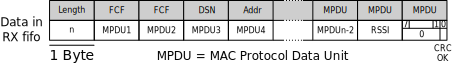
\includegraphics[width=0.6\columnwidth]{rx_fifo_content}
	\caption{The contents of RX fifo}
	\label{fig:rx_fifo_content}
\end{figure}


\hangindent=\parindent
\hangafter=0
Figure~\ref{fig:rx_fifo_content} shows the contents stored in RX fifo. The last two bytes
stored in the RX fifo are RSSI and CRC OK respectively. The RSSI value is unsigned 8 bytes
value. As mentioned before, the step size of RSSI is 14.8~mV. (eg: 137 = 2.03~V in RSSI)
CRC OK is a single bit in last byte. This bit is asserted if the packet passed CRC check
and vice versa.

\subsubsection{TX fifo}
\hangindent=\parindent
\hangafter=0
The depth and width of TX fifo is 128 and 8-bits respectively. In contrast to RX fifo, 
TX fifo contains only 1 packet every time. Transmitter loads preamble
and SFD automatically, which occupy 5 bytes in depth. Thus, the truly available depth for
user is $128 - 5 - 1$ (length) $= 122$ bytes. User only loads the "data" to TX fifo. The 
transmitter will automatically calculate corresponding FCS and appending it to the end
of TX fifo. 

\subsubsection{ACK fifo}
\hangindent=\parindent
\hangafter=0
\sdr support hardware ACK (HACK). Parts of ACK frame is pre-stored in ACK fifo. Once the received packet
has ACK request bit set, its DSN is passed to ACK fifo and fifo control starts calculating the FCS
for ACK frame. User cannot access to ACK fifo directly.

\subsubsection{FWD fifo}
\hangindent=\parindent
\hangafter=0
\sdr supports hardware packet forwarding. Receiver stores the decoded data into 2 different fifos - 
RX fifo and FWD fifo. However, the data stored in these fifos are slightly different in DSN field
and FCS. \sdr uses DSN as a relay counter to prevent the forwarding packet last forever in the network.
Only the packet has DSN which is less than threshold (0x7f) will be forwarded. Similar to TX fifo,
FWD fifo is not able to be accessed by user.

\clearpage
\subsection{Address Map}
\begin{table*}[h]
\centering
\begin{threeparttable}
	\begin{tabular}{|c|c|c|c|c|}
		\hline
		{\bf Address} & {\bf Width} & {\bf Bit Position} & {\bf Direction} & {\bf Registers} \\ \hline
		0x40050000 & 8  & 7:0 	& R		& RX fifo\\ \hline
		0x40050004 & 16 & 31:16 & R		& Src Pan ID\tnote{a}\\
		0x40050004 & 16 & 15:0	& R		& Dest Pan ID\tnote{a}\\ \hline
		0x4005000c & 1	& 18	& R		& RX fifo empty\\
		0x4005000c & 1	& 17	& R		& ACK set\tnote{a}\\
		0x4005000c & 1	& 16	& R		& CRC correct\tnote{a}\\
		0x4005000c & 16 & 15:0	& R		& FCF\tnote{a}\\ \hline
		0x40050010 & 32 & 31:0	& R		& Src address LSB\tnote{a}\\ \hline
		0x40050014 & 32 & 31:0	& R		& Src address MSB\tnote{a}\\ \hline
		0x40050018 & 32 & 31:0	& R		& Dest address LSB\tnote{a}\\ \hline
		0x4005001c & 32 & 31:0	& R		& Dest address MSB\tnote{a}\\ \hline\hline
		0x40060000 & 8	& 7:0	& W		& TX fifo\\ \hline\hline
		0x40070000 & 1	& 8		& R/W	& Auto TX en\\
		0x40070000 & 4	& 7:4	& R		& Radio mode\\
		0x40070000 & 1	& 3		& R/W	& ACK en\\
		0x40070000 & 2	& 2:1	& R/W	& AGC mode\\
		0x40070000 & 1	& 0		& R/W	& Radio off/on\\ \hline
		0x40070020 & 8	& 7:0	& R/W	& LED\\ \hline
		0x40070050 & 1	& 0		& W		& ACK flush\\ \hline\hline
		0x40080000 & 14	& 13:0	& W		& MAX2831 Register 0\tnote{b}\\ \hline
		0x40080004 & 14	& 13:0	& W		& MAX2831 Register 1\tnote{b}\\ \hline
		0x40080008 & 14	& 13:0	& W		& MAX2831 Register 2\tnote{b}\\ \hline
		0x4008000c & 14	& 13:0	& W		& MAX2831 Register 3\tnote{b}\\ \hline
		0x40080010 & 14	& 13:0	& W		& MAX2831 Register 4\tnote{b}\\ \hline
		0x40080014 & 14	& 13:0	& W		& MAX2831 Register 5\tnote{b}\\ \hline
		0x40080018 & 14	& 13:0	& W		& MAX2831 Register 6\tnote{b}\\ \hline
		0x4008001c & 14	& 13:0	& W		& MAX2831 Register 7\tnote{b}\\ \hline
		0x40080020 & 14	& 13:0	& W		& MAX2831 Register 8\tnote{b}\\ \hline
		0x40080024 & 14	& 13:0	& W		& MAX2831 Register 9\tnote{b}\\ \hline
		0x40080028 & 14	& 13:0	& W		& MAX2831 Register 10\tnote{b}\\ \hline
		0x4008002c & 14	& 13:0	& W		& MAX2831 Register 11\tnote{b}\\ \hline
		0x40080030 & 14	& 13:0	& W		& MAX2831 Register 12\tnote{b}\\ \hline
		0x40080034 & 14	& 13:0	& W		& MAX2831 Register 13\tnote{b}\\ \hline
		0x40080038 & 14	& 13:0	& W		& MAX2831 Register 14\tnote{b}\\ \hline
		0x4008003c & 14	& 13:0	& W		& MAX2831 Register 15\tnote{b}\\ \hline
	\end{tabular}
	\begin{tablenotes}
		%\small
		\item [a] Information is only valid for the last received packet.
		\item [b] Refer to datasheet~\cite{MAX2831} for detail information.
	\end{tablenotes}
\end{threeparttable}
\end{table*}

\clearpage
\section{Radio Operations}
\subsection{Receiving}
Once the radio is on, it normally resides in {\bf Idle Listening} mode. Once a packet arrives,
various interrupts are generated by receiver. User is able to respond toward different events.
Reading the received data is straightforward. User just need to keep reading the RX fifo address.
If the reading is performed in packet basis, the first byte readed out by user is usually the packet
length. Thus, user can initiate the PDMA transfer for the rest of the packet.

The receiver performs simple frame filtering. Thus, the address related fields are extracted 
and able to be read through AHB interface directly. However, user has to note that the information
is only valid for the last received packet. Also, any transmission (including ACK/Forward) put the 
receiver into reset reset, which flushes the registers' values.

\subsection{Transmitting}
Loading the data into TX fifo, user simply write to the TX fifo address. It's not necessary to initiate
the transmission after the TX fifo is completed filled. User can load the data into TX fifo while
the radio is currently transmitting. In order to initiate the
data transmission, user has to assert a GPIO which connects to the transmitter. However, the radio
is able to start transmitting only if the radio in the {\bf Idle Listening}. Therefore, user has
to check current radio state before asserting the GPIO line. Two methods are available to check the
current radio state.
\begin{enumerate}
	\item Radio mode register (0x40070000)
	\item GPIO inputs
\end{enumerate}
By accessing the radio mode register, user is able to identify the current radio mode. If current
radio mode is {\bf 0}, user is able to assert GPIO line. In addition, "ready\_to\_transmit" signal is 
connected to an MSS GPIO line, which is another indicator to initate the transmission.

User has to be aware that the exact timing for radio start transmitting is not the time when GPIO
has been asserted. Since radio normally in the {\bf Idle Listening} mode, it takes time for the
RF frontend to switch its mode from RX to TX. In \sdr, the time between GPIO asserts and actually
transmitted is 2~$\mu$s.

If precise timing is required, \sdr offers a fixed timing (192~$\mu$s) auto transmission. If the
{\bf "Auto TX enable"} is asserted, radio starts transmitting after 192~$\mu$s of a packet is received.
Automatic transmission is useful in concurrent transmission scenario.

\subsection{ACK}
\sdr supports hardware ACK. By default, \sdr has Auto ACK enabled. User can disable the Auto ACK by
deasserting the ACK en register. The ACK frame has to be sent right after 192~$\mu$s if {\bf all} the 
following conditions are met.
\begin{enumerate}
	\item ACK request field is set
	\item Packet passes CRC
	\item Destination address match radio's address
\end{enumerate}
\sdr is designed to support multiple address recognition. However, the address field in 802.15.4
standard could be 8 bytes long. Giving the space constraint, the address recognition is moved to
processor. Therefore, the processor must complete the 3rd condition within 192~$\mu$s. If a
packet meets the first two conditions, fabric starts preparing the ACK frame and initiating a
down counter. If destination address doesn't match to radio's address, processor has to "flush"
the outgoing ACK. "Flush" can be done by asserting the ACK flush register (0x40070050).

\subsection{Forwarding}
\sdr supports hardware forwarding. The forwarding is entirely built in fabric. Thus no processor
is required. The packet is been forwarded if {\bf all} the following conditions are met.
\begin{enumerate}
	\item Destination address is equal to 0xfffe or 0xffff\_ffff\_ffff\_fffe (depends on destination 
	address mode)
	\item DSN is less than 127
	\item Packet passes CRC
\end{enumerate}
The fabric increments its DSN and updating its FCS for each forwarding packet. The packet will be
forwarded after 192~$\mu$s

\subsection{Automatic Gain Control (AGC)}
MAX2831 RF frontend doesn't provide AGC in package. However, user can set fixed gain through SPI
interface or enabling the AGC in fabric. The detail of RX gain setting can be found in MAX2831
datasheet Table 26~\cite{MAX2831}. To enable the AGC in Fabric, user has to write to AGC mode 
register. Two different AGC mode is available.

\begin{table}[h]
\centering
	\begin{tabular}{|c|c|l|}
	\hline
	{\bf AGC mode register} & {\bf AGC Mode} & {\bf Description} \\ \hline
	0 & Off & AGC is disabled\\ \hline
	1 & SFD-Latched & Gain setting is latched by the SFD detection\\ \hline
	2 & Reserved & Reserved\\ \hline
	3 & Contiuous & Gain setting keeps adapting to signal strength\\ \hline
	\end{tabular}
\end{table}

\section{Interrupts and Pin Activity}
\subsection{Receiving}
Several critical pins are connected to MSS GPIO, which allows user to monitor and responding
to radio events. In the receiving mode, SFD pin goes high after radio successfully decoded
SFD field in the packet. Similarly, Length pin goes high after {\bf valid length}~\footnote{
In 802.15.4 standard, the length field should be greater or equal to 5 and less or equal to 127} 
field has been decoded. Once the length field is corrupted, radio back to wait preamble
and the SFD pin deasserts. Figure~\ref{fig:pin_activity_rx} shows a "complete" interrupt is added
to the \sdr. The "complete" interrupt is a pulse signal, which asserts after a packet reception
has been complete and deassert after 62.5~$\mu$s.
\begin{figure}[h]
\centering
	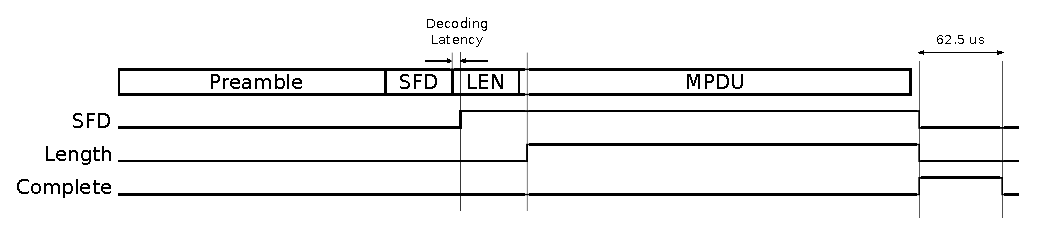
\includegraphics[width=0.96\columnwidth]{pin_activity_rx}
	\caption{Pins activity during receiving}
	\label{fig:pin_activity_rx}
\end{figure}
Since the SmartFusion has PDMA integrated, user can configure the complete as a interrupt to 
processor. Once the complete interrupt arrived, a PDMA transfer unloads the entire packet to
processor.

\subsection{Transmitting}
Similarly, PDMA also benefits the data loading process. User can initiate a PDMA transfer to
load the entire packet into TX fifo. Note that user can start TX transmit without waiting
the DMA transfer completed. Once the TX fifo is empty, a TX complete interrupt asserts.
The signal indicates user is able to load the next packet.
\begin{figure}[h]
\centering
	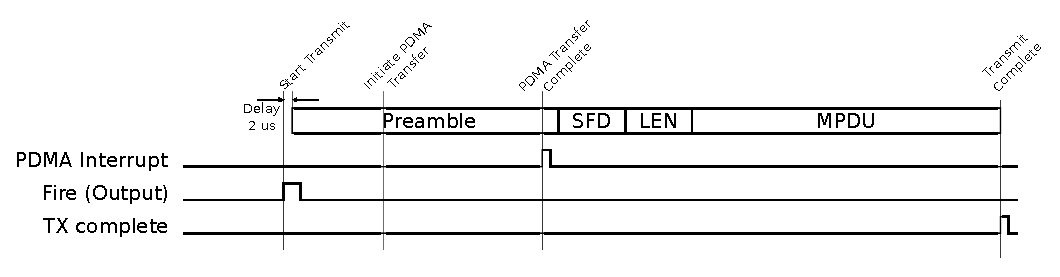
\includegraphics[width=0.9\columnwidth]{pin_activity_tx}
	\caption{Interrupts activity during transmitting}
	\label{fig:pin_activity_tx}
\end{figure}
Figure~\ref{fig:pin_activity_tx} shows the interrupts activity. In this example, "Fire" is a MSS GPIO
output which connects to the fabric. User asserts Fire to start transmitting the packet. It is not necessary
to upload the packet before Fire assert. However, data must be start loading before SFD has been transmitted.

\begin{table}[h]
\centering
	\begin{tabular}{|c|c|}
	\end{tabular}
\end{table}

\section{Drivers}
\subsection{max2831}
The following functions are provided in the max2831 driver. Although the MAX2831 internal registers'
cannot be read through SPI interface, the driver maintains the registers' values. User can retrieves
these value through a provided function.

\begin{enumerate}
	\item void initialize\_chip();
	\item void setToDefaultRX(int register\_number);
	\item void setRegisterValueRX(int register\_number,uint32\_t register\_value);
	\item uint32\_t getRegisterValueRX(int reg\_number);
	\item uint8\_t setLNAGain(uint8\_t LNAGain);
	\item uint8\_t setRXBaseBandVGAGain(uint8\_t VGAGain);
	\item uint8\_t setTXBaseBandVGAGain(uint8\_t VGAGain);
	\item void enRXParVGAGainCtl();
	\item uint8\_t setFreqDivider(int freq);
	\item int getFreqDivider();
	\item uint8\_t setBaseBandLowPassFilterMode (uint8\_t LPFMode);
	\item uint8\_t setTXBaseBandLowPassFilterModeFineAdjust (uint8\_t LPFMode, uint8\_t LPFFineAdjust);
	\item uint8\_t setRXBaseBandLowPassFilterModeFineAdjust (uint8\_t LPFMode, uint8\_t LPFFineAdjust);
\end{enumerate}

\subsubsection{void initialize\_chip()}
\hangindent=\parindent
\hangafter=0
Input argument: None\\
Return value: None\\
This function resets all registers to the default value.

\subsubsection{void setToDefaultRX(int register\_number)}
\hangindent=\parindent
\hangafter=0
Input argument: Register number. A valid register number is from 0 to 15.\\
Return value: None\\
This function sets the specified register to its default value.

\subsubsection{void setRegisterValueRX(int register\_number,uint32\_t register\_value)}
\hangindent=\parindent
\hangafter=0
Input argument: Register number, Register value. A valid register number is from 0 to 15.\\
Return value: None\\
This function set the specified register to specified value.

\subsubsection{uint32\_t getRegisterValueRX(int reg\_number)}
\hangindent=\parindent
\hangafter=0
Input argument: Register number. A valid register number is from 0 to 15.\\
Return value: Register value\\
This function returns the specified register's value.

\subsubsection{uint8\_t setLNAGain(uint8\_t LNAGain)}
\hangindent=\parindent
\hangafter=0
Input argument: LNA gain. A valid LNA gain is from 0 to 3.\\
Return value: Success/Fail. 0: Fail, 1: Success.\\
This function sets the LNA gains in RX loop and return success/fail.
\begin{table}
\centering
	\begin{tabular}{|c|c|}
		\hline
		{\bf LNA Gain} & {\bf Mode}\\ \hline
		0 or 1 & Low gain\\ \hline
		2 & Medium gain\\ \hline
		3 & High gain\\ \hline
	\end{tabular}
	\caption{LNA gain mode}
\end{table}

\subsubsection{uint8\_t setRXBaseBandVGAGain(uint8\_t VGAGain)}
\hangindent=\parindent
\hangafter=0
Input argument: VGA gain. A valid VGA gain is from 0 (min) to 31 (max). Step size = 2~dB\\
Return value: Success/Fail. 0: Fail, 1: Success.\\
This function sets the {\bf RX} baseband gain.

\subsubsection{uint8\_t setTXBaseBandVGAGain(uint8\_t VGAGain)}
\hangindent=\parindent
\hangafter=0
Input argument: VGA gain. A valid VGA gain is from 0 (min) to 63 (max). Step size = 2~dB\\
Return value: Success/Fail. 0: Fail, 1: Success.\\
This function set the {\bf TX} baseband gain.

\subsubsection{void enRXParVGAGainCtl()}
\hangindent=\parindent
\hangafter=0
Input argument: None\\
Return value: None\\
This function enables the parallel control over the RX gain. It's necessary for AGC and Only 
valid on \sdr v2.

\subsubsection{uint8\_t setFreqDivider(int freq)}
\hangindent=\parindent
\hangafter=0
Input argument: RF Frequency\\
Return value: Success/Fail. 0: Fail, 1: Success.\\
This function sets the RF frequency of MAX2831.

\subsubsection{int getFreqDivider()}
\hangindent=\parindent
\hangafter=0
Input argument: None\\
Return value: RF frequency
This function returns the RF frequency of MAX2831.

\begin{comment}
\subsubsection{uint8\_t setBaseBandLowPassFilterMode (uint8\_t LPFMode)}
\hangindent=\parindent
\hangafter=0
Input argument: Low Pass Filter Mode\\
Return value: Success/Fail. 0: Fail, 1: Success.\\
\end{comment}

\subsubsection{uint8\_t setTXBaseBandLowPassFilterModeFineAdjust (uint8\_t LPFMode, uint8\_t LPFFineAdjust)}
\hangindent=\parindent
\hangafter=0
Input argument: Low Pass Filter Mode, Adjustment\\
Return value: Success/Fail. 0: Fail, 1: Success.\\
See table~\ref{tab:lpf} for more details.

\subsubsection{uint8\_t setRXBaseBandLowPassFilterModeFineAdjust (uint8\_t LPFMode, uint8\_t LPFFineAdjust)}
\hangindent=\parindent
\hangafter=0
Input argument: Low Pass Filter Mode, Adjustment\\
Return value: Success/Fail. 0: Fail, 1: Success.\\
See table~\ref{tab:lpf} for more details.

\begin{table}[h]
\centering
	\begin{tabular}{|c|c|c|c|c|c|c|c|c|c|c|c|}
	\hline
	\multirow{3}{*}{LPF Mode} &
	\multicolumn{11}{c|}{LPF Fine Adjustment}\\ \cline{2-12}
	& \multicolumn{5}{c|}{RX} &
	\multicolumn{6}{c|}{TX} \\ \cline{2-12}
			& {\bf 0} & {\bf 1} & {\bf 2} & {\bf 3} & {\bf 4} & {\bf 0} & {\bf 1} & {\bf 2} & {\bf 3} & {\bf 4} & {\bf 5}\\ \hline
	{\bf 0} & \multirow{4}{*}{90\%} & \multirow{4}{*}{95\%} & 7.5~MHz & \multirow{4}{*}{105\%} & \multirow{4}{*}{110\%} 
			& \multirow{4}{*}{90\%} & \multirow{4}{*}{95\%} & 8~MHz   & \multirow{4}{*}{105\%} & \multirow{4}{*}{110\%} & \multirow{4}{*}{115\%}\\ \cline{1-1}\cline{4-4}\cline{9-9}
	{\bf 1} &  &  & 8.5~MHz &  &  &  &  & 11~MHz	&  &  & \\ \cline{1-1}\cline{4-4}\cline{9-9}
	{\bf 2} &  &  & 15~MHz 	&  &  &  &  & 16.5~MHz	&  &  & \\ \cline{1-1}\cline{4-4}\cline{9-9}
	{\bf 3} &  &  & 18~MHz 	&  &  &  &  & 22.5~MHz	&  &  & \\ \hline
	\end{tabular}
	\caption{LPF adjustment details}
	\label{tab:lpf}
\end{table}


\subsection{tx\_packet}
The {\bf tx\_packet\_str} is a abstraction of a TX packet structure. 
Most of the functions are used to set the FCF field in TX packet. FCF has two bytes in length
and each bits represent different information. Figure~\ref{fig:FCF} gives a brief view of FCF
field. A tx packet contains header and payloads. {\bf tx\_packet\_str } stores most of the header 
information except the {\bf source address}, {\bf source address mode} and {\bf source PAN ID}.
These information can be retrieved by a pointer to a radio ({\bf rp}) structure which owns this 
tx packet. Also, {\bf data\_ptr} is the pointer to the payload.
\begin{figure}[h]
	\centering
	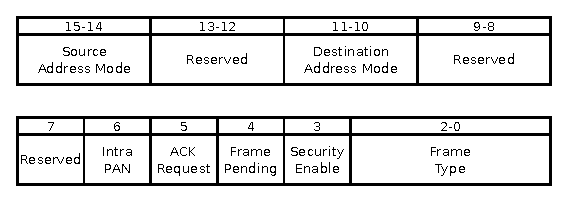
\includegraphics[width=0.6\columnwidth]{FCF}
	\caption{Detail information of FCF field}
	\label{fig:FCF}
\end{figure}

\begin{lstlisting}[language=c, caption=TX Packet Structure]
	struct tx_packet_str{
		uint8_t frame_type;
		uint8_t security_en;
		uint8_t frame_pending;
		uint8_t ack_req;
		uint8_t intra_pan;
		uint8_t dest_addr_mode;
		uint8_t dsn;
		uint16_t dest_pan_ID;
		uint32_t dest_addr_LSB, dest_addr_MSB;
		uint8_t pkt_overhead;
	
		uint8_t data_length;
		uint32_t* data_ptr;
		struct radio* rp;
	};
\end{lstlisting}

\begin{enumerate}
	\item inline uint8\_t set\_dest\_addr\_mode(struct tx\_packet\_str* tp, uint8\_t dam);
	\item inline void set\_pan\_id\_comp(struct tx\_packet\_str* tp, uint8\_t ip);
	\item inline void set\_ack(struct tx\_packet\_str* tp, uint8\_t ar);
	\item inline void set\_frame\_pending(struct tx\_packet\_str* tp, uint8\_t fp);
	\item inline void set\_security(struct tx\_packet\_str* tp, uint8\_t se);
	\item inline void set\_frame\_type(struct tx\_packet\_str* tp, uint8\_t ft);
	\item inline void set\_DSN(struct tx\_packet\_str* tp, uint8\_t DSN);
	\item inline void set\_dest\_pan(struct tx\_packet\_str* tp, uint16\_t dp);
	\item inline void set\_dest\_addr(struct tx\_packet\_str* tp, uint32\_t da1, uint32\_t da0);
	\item void calculate\_FCF(struct tx\_packet\_str* tp, uint32\_t* tx\_pkt\_ptr);
	\item uint8\_t calculate\_address(struct tx\_packet\_str* tp, uint32\_t* tx\_pkt\_ptr);
	\item uint8\_t data\_trans (struct tx\_packet\_str* tp);
\end{enumerate}

\subsubsection{inline uint8\_t set\_dest\_addr\_mode(struct tx\_packet\_str* tp, uint8\_t dam)}
\hangindent=\parindent
\hangafter=0
Input argument: tx\_packet\_str pointer, destination address mode (dam).\\
Return value: Success/Fail. 0: Fail, 1: Success.\\
\begin{table}[h]
\centering
	\begin{tabular}{|c|c|}
	\hline
	{\bf Source/Destination Address Mode} & {\bf Address Field Length}\\ \hline
	0 & No PAN/Address present\\ \hline
	2 & 2 Bytes\\ \hline
	3 & 8 Bytes\\ \hline
	\end{tabular}
	\caption{List of destination address mode}
	\label{tab:address_mode}
\end{table}

\subsubsection{inline void set\_pan\_id\_comp(struct tx\_packet\_str* tp, uint8\_t ip)}
\hangindent=\parindent
\hangafter=0
Input argument: tx\_packet\_str pointer, Intra PAN (ip)\\
Return value: None\\
"The PAN ID Compression subfield is 1 bit in lengthand specifies whether the MAC frame is to 
be sent containing only one of the PAN identifier fields whenboth source and destination 
addresses are present"~\cite{802.15.4.standard}
The available options are following:
\begin{table*}[h]
\centering
\begin{threeparttable}
	\begin{tabular}{|c|c|c|c|c|}
	\hline
	{\bf Intra PAN} & {\bf Dest. PAN} & {\bf Dest. Addr.} & {\bf Source PAN} & {\bf Source Addr.}\\ \hline
	1 & Present			& Present			& None~\tnote{a}	& Present\\ \hline
	0 & Present			& Present			& Present			& Present\\ \hline
	0 & Present			& Present			& None~\tnote{b}	& None~\tnote{b}\\ \hline
	0 & None~\tnote{b}	& None~\tnote{b}	& Present			& Present\\ \hline
	0 & None~\tnote{b}	& None~\tnote{b}	& None~\tnote{b}	& None~\tnote{b}\\ \hline
	\end{tabular}
	\begin{tablenotes}
		\item [a] Source PAN ID. equals to Destination PAN ID.
		\item [b] Refer table~\ref{tab:address_mode} for detail information.
	\end{tablenotes}
\end{threeparttable}
	\caption{PAN ID compression and source/destination address mode}
\end{table*}

\subsubsection{inline void set\_ack(struct tx\_packet\_str* tp, uint8\_t ar)}
\hangindent=\parindent
\hangafter=0
Input argument: tx\_packet\_str pointer, ACK request (ar)\\
Return value: None\\
\begin{table}[h]
\centering
	\begin{tabular}{|c|c|}
	\hline
	{\bf ACK request (ar)} & {\bf Effect}\\ \hline
	0 & No ACK\\ \hline
	1 & Request ACK\\ \hline
	\end{tabular}
	\caption{ACK Request}
\end{table}
Note that the ACK request bit should not be set in broadcast~\footnote{
Destination address \= 0xffff or 0xffffffffffffffff} packet.


\subsubsection{inline void set\_frame\_pending(struct tx\_packet\_str* tp, uint8\_t fp)}
\hangindent=\parindent
\hangafter=0
Input argument: tx\_packet\_str pointer, frame pending(fp)\\
Return value: None\\
\begin{table}[h]
\centering
	\begin{tabular}{|c|c|}
	\hline
	{\bf frame pending (fp)} & {\bf Effect}\\ \hline
	0 & No frame pending\\ \hline
	1 & Frame pending\\ \hline
	\end{tabular}
	\caption{Frame Pending}
\end{table}

\subsubsection{inline void set\_security(struct tx\_packet\_str* tp, uint8\_t se)}
\hangindent=\parindent
\hangafter=0
Input argument: tx\_packet\_str pointer, Security Enable (se)\\
Return value: None\\
\begin{table}[h]
\centering
	\begin{tabular}{|c|c|}
	\hline
	{\bf Security Enable (se)} & {\bf Effect}\\ \hline
	0 & Security Enable\\ \hline
	1 & Security Disable\\ \hline
	\end{tabular}
	\caption{Security enable}
\end{table}

\subsubsection{inline void set\_frame\_type(struct tx\_packet\_str* tp, uint8\_t ft)}
\hangindent=\parindent
\hangafter=0
Input argument: tx\_packet\_str pointer, Frame Type (ft)\\
Return value: None\\
\begin{table}[h]
\centering
	\begin{tabular}{|c|c|}
	\hline
	{\bf Frame Type (ft)} & {\bf Effect}\\ \hline
	0 & Beacon\\ \hline
	1 & Data\\ \hline
	2 & Acknowledgment\\ \hline
	3 & Mac Command\\ \hline
	\end{tabular}
	\caption{Frame type}
\end{table}

\subsubsection{inline void set\_DSN(struct tx\_packet\_str* tp, uint8\_t DSN)}
\hangindent=\parindent
\hangafter=0
Input argument: tx\_packet\_str pointer, Data Sequence Number (DSN)\\
Return value: None\\
This function sets the DSN field in a TX packet.


\subsubsection{inline void set\_dest\_pan(struct tx\_packet\_str* tp, uint16\_t dp)}
\hangindent=\parindent
\hangafter=0
Input argument: tx\_packet\_str pointer, Destination PAN ID (dp)\\
Return value: None\\
This function sets the destination PAN ID in a TX packet.


\subsubsection{inline void set\_dest\_addr(struct tx\_packet\_str* tp, uint32\_t da1, uint32\_t da0)}
\hangindent=\parindent
\hangafter=0
Input argument: tx\_packet\_str pointer, Destination Address (da1, da0)\\
Return value: None\\
This function sets the destination address in a TX packet. Destination address could be as
long as 8 bytes (destination address mode = 3). If 8 bytes mode is selected, destination
address = {da1 (higher 32-bits), da0 (lower 32-bits)}. Similarly, destination address = 
(da0 \& 0xffff) if 2 bytes mode is selected.

\subsubsection{void calculate\_FCF(struct tx\_packet\_str* tp, uint32\_t* tx\_pkt\_ptr)}
\hangindent=\parindent
\hangafter=0
Input argument: tx\_packet\_str pointer, TX packet header pointer\\ 
Return value: None\\
This function aggregates all the settings to 2 bytes FCF field.

\subsubsection{uint8\_t calculate\_address(struct tx\_packet\_str* tp, uint32\_t* tx\_pkt\_ptr)}
\hangindent=\parindent
\hangafter=0
Input argument: tx\_packet\_str pointer, TX packet header pointer\\ 
Return value: 
This function calculates address format in a TX packet by source/destination
address mode and Intra PAN ID bit.

\subsubsection{uint8\_t data\_trans (struct tx\_packet\_str* tp)}
\hangindent=\parindent
\hangafter=0
Input argument: tx\_packet\_str pointer\\ 
Return value: Success/Fail. 0: Fail, 1: Success.\\
This function initiates a PDMA transfer which load the packet into TX fifo.

\subsection{rx\_packet}
This driver is a "reverse" operation of tx\_packet. The driver extracts the parameters in header
from a received packet. The following source code is the {\bf rx\_packet\_str} structure. It's
very similar to tx\_packet\_str. The major diferences are the source address information,
rssi value and crc result.

\begin{lstlisting}[caption=RX Packet Structure]
struct rx_packet_str{
	uint8_t frame_type;
	uint8_t security_en;
	uint8_t frame_pending;
	uint8_t ack_req;
	uint8_t intra_pan;
	uint8_t dest_addr_mode;
	uint8_t dsn;
	uint16_t dest_pan_ID;
	uint32_t dest_addr_LSB, dest_addr_MSB;

	uint8_t packet_length;
	uint32_t payload_idx;

	uint8_t src_addr_mode;
	uint16_t src_pan_ID;
	uint32_t src_addr_LSB, src_addr_MSB;
	uint8_t rssi;
	uint8_t crc;
};
\end{lstlisting}

\begin{enumerate}
	\item void read\_fifo(uint32\_t* rdata);
	\item inline uint8\_t isFifoEmpty();
	\item uint8\_t rx\_packet\_create(struct rx\_packet\_str* rp, uint32\_t* rx\_data);
\end{enumerate}

\subsubsection{void read\_fifo(uint32\_t* rdata)}
\hangindent=\parindent
\hangafter=0
Input argument: A pointer where stores the unloaded data.\\
Return value: None\\
This function unload {\bf one packet}~\footnote{Only the oldest packet in RX fifo.} from RX fifo. 
The unloaded data will be stored in {\bf rdata} array. The size of rdata cannot be too small to
store a single packet.

\subsubsection{inline uint8\_t isFifoEmpty()}
\hangindent=\parindent
\hangafter=0
Input argument: None\\
Return value: Fifo empty\\
This function checks whether the RX fifo is empty or not. If it's empty, function returns 1 and
vice versa.

\subsubsection{uint8\_t rx\_packet\_create(struct rx\_packet\_str* rp, uint32\_t* rx\_data)}
\hangindent=\parindent
\hangafter=0
Input argument: rx\_packet\_str pointer, a pointer where stores the unloaded data.\\
Return value: Success/Fail. 0: Fail, 1: Success.\\
This function extracts and stores all the data member in rx\_packet\_str from a given rx\_data
pointer. 

\clearpage
\subsection{radio\_config}
This driver provides the low-level radio hardware configuration and source address information.
The radio structure below shows its data member. All the data member are address correlated.
User has to note that the fabric doesn't perform the address recognition because of the area
constraint. In order for the radio to operate properly, user has to perform address recoginition
in time. In addition, multiple source addresses is supported by software configuration. 

\begin{lstlisting}[caption=Radio Structure]
struct radio{
	uint8_t multiple_addr_en;
	uint8_t num_of_multiple_addr;
	uint32_t* multiple_addr_ptr;
	uint16_t src_pan_ID;
	uint8_t src_addr_mode;
	uint32_t src_addr_LSB, src_addr_MSB;
};
\end{lstlisting}

\begin{enumerate}
	\item void init\_system();
	\item inline void tx\_fire();
	\item void RF\_shdn(uint8\_t shdn);
	\item inline void auto\_ack\_en(uint8\_t ack\_en);
	\item inline void rx\_agc\_en(uint8\_t agc\_mode);
	\item inline void ack\_flush();
	\item inline void auto\_tx\_en(uint8\_t en);
	\item uint8\_t get\_radio\_mode();
	\item uint8\_t dest\_addr\_filter(struct rx\_packet\_str* rp, struct radio* r0);
	\item void set\_multiple\_address(struct radio* r0, uint8\_t en, uint8\_t nu, uint32\_t* map);
	\item inline uint8\_t set\_src\_addr\_mode(struct radio* r0, uint8\_t sam);
	\item inline void set\_src\_pan(struct radio* r0, uint16\_t sp);
	\item inline void set\_src\_addr(struct radio* r0, uint32\_t sa1, uint32\_t sa0);
\end{enumerate}


\subsubsection{void init\_system()}
\hangindent=\parindent
\hangafter=0
Input argument: None\\
Return value: None\\
This function initialize the entire radio including MAX2831, GPIO and PDMA drivers. This function
should be called before any other radio correlated functions.

\subsubsection{inline void tx\_fire()}
\hangindent=\parindent
\hangafter=0
Input argument: None\\
Return value: None\\
This function starts transmitting the content of TX fifo.

\subsubsection{void RF\_shdn(uint8\_t shdn)}
\hangindent=\parindent
\hangafter=0
Input argument: radio shutdown\\
Return value: None\\
This function turns off all the radio peripherals. (RF, ADCs and DAC)

\subsubsection{inline void auto\_ack\_en(uint8\_t ack\_en)}
\hangindent=\parindent
\hangafter=0
Input argument: ACK enable/disable\\
Return value: None\\
\begin{table}[h]
\centering
	\begin{tabular}{|c|c|}
	\hline
		{\bf Auto ACK en (ack\_en)} & {\bf Effect}\\ \hline
		0 & Disable Auto ACK\\ \hline
		1 & Enable Auto ACK\\ \hline
	\end{tabular}
	\caption{ACK Enable/Disable}
\end{table}


\subsubsection{inline void rx\_agc\_en(uint8\_t agc\_mode)}
\hangindent=\parindent
\hangafter=0
Input argument: AGC mode\\
Return value: None\\
\begin{table}[h]
\centering
	\begin{tabular}{|c|c|}
	\hline
		{\bf AGC mode (agc\_mode)} & {\bf Effect}\\ \hline
		0 & Disable AGC\\ \hline
		1 & SFD-Latch AGC\\ \hline
		2 & Reserved\\ \hline
		3 & Continues AGC\\ \hline
	\end{tabular}
	\caption{AGC Mode}
\end{table}

\subsubsection{inline void ack\_flush()}
\hangindent=\parindent
\hangafter=0
Input argument: None\\
Return value: None\\
This function flushes the outgoing ACK packet. Once a packet reception completed, user should
unload the packet from the radio and perform destination address filter. It returns whether
the address is match to radio's source address or not. In the mean time, user needs to check
the coming packet has ACK request bit set or not. If the following conditions are met, user
should call ack\_flush();
\begin{enumerate}
	\item Destination address {\bf doesn't} match to local source address.
	\item Packet passes the CRC check.
	\item Packet has ACK request field set.
\end{enumerate}

\subsubsection{inline void auto\_tx\_en(uint8\_t en)}
\hangindent=\parindent
\hangafter=0
Input argument: Auto TX enable\\
Return value: None\\
This function enables the automatic transmission of TX fifo. User can achieve concurrent
transmission using this function.
\begin{table}[h]
\centering
	\begin{tabular}{|c|c|}
	\hline
		{\bf Auto TX enable (en)} & {\bf Effect}\\ \hline
		0 & Disable Auto TX\\ \hline
		1 & Radio starts transmitting after 192~$\mu$s of any packet received\\ \hline
	\end{tabular}
	\caption{Auto TX}
\end{table}

\subsubsection{uint8\_t get\_radio\_mode()}
\hangindent=\parindent
\hangafter=0
Input argument: None\\
Return value: Radio mode\\
This function is mainly used for debugging purpose.
\begin{table}[h]
\centering
	\begin{tabular}{|c|c|c|}
	\hline
		{\bf Radio Mode} & {\bf Fabric State} & {\bf Corresponding State}\\ \hline
		0x00 & RX\_IDLE & Idle Listening\\ \hline
		0x01 & RX\_COLLECT & RX\\ \hline
		0x03 & TX\_RX\_TURNAROUND & \\ \hline
		0x04 & RX\_TX\_TURNAROUND & \\ \hline
		0x05 & RX\_WAIT\_FOR\_ACK\_GLOSSY & \\ \hline
		0x08 & RADIO\_OFF & Off\\ \hline
		0x09 & RADIO\_WARMUP & \\ \hline
		0x0c & WAIT\_FOR\_TX\_COMPLETE & TX\\ \hline
		0x0d & RX\_WAIT\_FOR\_ACK\_GLOSSY\_COMPLETE & \\ \hline
	\end{tabular}
	\caption{Radio Mode}
\end{table}


\subsubsection{uint8\_t dest\_addr\_filter(struct rx\_packet\_str* rp, struct radio* r0)}
\hangindent=\parindent
\hangafter=0
Input argument: rx\_packet\_str pointer, radio struct pointer\\
Return value: Match/Mismatch. 0: Mismatch, 1: Match.\\

\subsubsection{void set\_multiple\_address(struct radio* r0, uint8\_t en, uint8\_t nu, uint32\_t* map)}
\hangindent=\parindent
\hangafter=0
Input argument: radio struct pointer, multiple address enable, 
number of multiple address, multiple address array\\
Return value: None\\

\subsubsection{inline uint8\_t set\_src\_addr\_mode(struct radio* r0, uint8\_t sam)}
\hangindent=\parindent
\hangafter=0
Input argument: radio struct pointer, Source Address Mode (sam)\\
Return value: Success/Fail. 0: Fail, 1: Success.\\
See table~\ref{tab:address_mode} for detail information.

\subsubsection{inline void set\_src\_pan(struct radio* r0, uint16\_t sp)}
\hangindent=\parindent
\hangafter=0
Input argument: radio struct pointer, Source PAN ID (sp)\\
Return value: None\\
This function sets the source PAN ID in a radio struct.

\subsubsection{inline void set\_src\_addr(struct radio* r0, uint32\_t sa1, uint32\_t sa0)}
\hangindent=\parindent
\hangafter=0
Input argument: radio struct pointer, Source Address (sa1, sa0)\\
Return value: None\\
This function sets the source address in a radio struct. Source address could be as
long as 8 bytes (source address mode = 3). If 8 bytes mode is selected, source  
address = {sa1 (higher 32-bits), sa0 (lower 32-bits)}. Similarly, source address = 
(sa0 \& 0xffff) if 2 bytes mode is selected.


\clearpage
\section{Example Codes (LED counter)}

\lstset{basicstyle=\footnotesize\ttfamily}
\begin{lstlisting}[caption=Initialize system]
	RF_shdn(0);
	init_system();
	res = setTXBaseBandVGAGain(10);
	uint32_t frequency = 2405;
	res = setFreqDivider(frequency);
	rx_agc_en(3);
\end{lstlisting}

\begin{lstlisting}[caption=Create object]

	struct radio* radio0;
	radio0 = malloc(sizeof(struct radio));
	radio0->multiple_addr_en = 0;		

	struct tx_packet_str* led_pkt;
	led_pkt = malloc(sizeof(struct tx_packet_str));
	// link to radio0
	led_pkt->rp = radio0;				

	struct rx_packet_str* received_packet;
	received_packet = malloc(sizeof(struct rx_packet_str));
\end{lstlisting}


\begin{lstlisting}[caption=Set packet \& Radio]
	uint32_t* led_data_ptr;
	uint32_t data_size = 4;
	led_data_ptr = malloc(sizeof(uint32_t)*data_size);
	led_pkt->data_length = data_size;
	led_pkt->data_ptr = led_data_ptr;

	// set led packet
	set_frame_type(led_pkt, 1);
	set_security(led_pkt, 0);
	set_pan_id_comp(led_pkt, 1);
	set_dest_addr_mode(led_pkt, 2);
	set_DSN(led_pkt, 0);
	set_dest_pan(led_pkt, 0x22);
	set_frame_pending(led_pkt, 0);

	set_dest_addr(led_pkt, 0, 0xffff);
	set_ack(led_pkt, 0);

	// set radio
	set_src_pan(radio0, 0x22);
	set_src_addr_mode(radio0, 2);
	set_src_addr(radio0, 0, 0x05);

	// set radio packet data
	led_data_ptr[0] = 0x3f;
	led_data_ptr[1] = 0x06;
	led_data_ptr[2] = 0x00;
	led_data_ptr[3] = 0x00;
\end{lstlisting}


\begin{lstlisting}[caption=Periodic transmit]
	if (TIM1_int & PDMA_int){
		tx_fire();
		PDMA_int = 0;
		TIM1_int = 0;
	}
\end{lstlisting}


\begin{lstlisting}[caption=Load packet]
	if (tx_complete_int==1){
		tx_complete_int = 0;
		tx_counter++;
		led_data_ptr[2] = (tx_counter & 0xff00)>>8;
		led_data_ptr[3] = (tx_counter & 0xff);
		set_DSN(led_pkt, led_data_ptr[3]);
		data_trans (led_pkt);
	}
\end{lstlisting}

\begin{lstlisting}[caption=Unload packet]
	if (rx_pkt_done_int==1){
		rx_pkt_done_int = 0;
		read_fifo(rdata);

		res = rx_packet_create(received_packet, rdata);

		uint8_t crc_correct, ack_req;
		crc_correct = received_packet->crc;
		ack_req = received_packet->ack_req;
		if (crc_correct){
			uint32_t* rx_data = rdata + received_packet->payload_idx;

			uint8_t address_match = dest_addr_filter(received_packet, radio0);

			// address doesn't match but requests ACK
			// flush ack
			if ( (!address_match) & ack_req){
				ack_flush();
			}

			// broadcast 
			if (address_match==3){
			// led packet signature, 0x3f, 0x06
				if ((rx_data[0]==0x3f)&&(rx_data[1]==0x06)){
					set_led(rx_data[3]);
				}
			}

		}

	}
\end{lstlisting}



\vfill\eject

% page limit          % 14.0 pg


%%%%%%%%%%%%%%%%%%%%%%%%%%%%%%%%%%%%
\clearpage
\section{Document Revision History}
\label{sec:revisions}

\begin{itemize}

\item Revision 0.2 {\footnotesize(rxxxx)} -- Feb 24, 2013
\subitem English/grammar corrections
\subitem Adding notes on todo items

\item Revision 0.1 {\footnotesize(r1525)} -- Sep 26, 2012
\subitem Initial revision

\end{itemize}


% abstract            % 0.5 pg
\vfill\eject

%\theendnotes

{%\footnotesize
\raggedright
\bibliographystyle{abbrv}
\bibliography{bib}
}

\end{document}

